\documentclass[a4paper,11pt]{article}
\usepackage[utf8]{inputenc}
\usepackage{amsmath}

% set up sensible margins (same as for cssethesis)
\usepackage[paper=a4paper,left=30mm,width=150mm,top=25mm,bottom=25mm]{geometry} 
\usepackage{cite} % Use the natbib bibliography and citation package
\usepackage{setspace} % This is used in the title page
\usepackage{graphicx} % This is used to load the crest in the title page
\usepackage{amsmath}
\usepackage{multicol}
\usepackage{color}
\usepackage{textcomp}
\usepackage{algpseudocode}
\usepackage{algorithm}
\usepackage{amssymb}
\usepackage{cleveref} 
\usepackage{epsfig}
%\usepackage[ruled, vlined]{algorithm2e}
\usepackage{epstopdf}
\usepackage{subfigure}
\usepackage{sectsty} 
\usepackage{amsmath}
\usepackage{qtree}
\usepackage{multirow}
\usepackage{lscape}
%\usepackage{refcheck}
%\usepackage[backref]{hyperref}
%\usepackage{hyperref}
%\usepackage{rotating}
%\usepackage{comment}


%\usepackage{enumerate}
%\usepackage[shortlabels]{enumitem}

\begin{document}


%\begin{enumerate}[start=1,label={(\bfseries Q\arabic*):}]

% Set up a title page
\thispagestyle{empty} % no page number on very first page
% Use roman numerals for page numbers initially
%\renewcommand{\thepage}{\roman{page}}

\begin{spacing}{1.5}
\begin{center}
\vspace*{5mm}
{\LARGE \bfseries
INDUSTRIAL TRAINING REPORT}
\medskip\\
\textbf{TRAINING MODULE FOR IN-HOUSE TRAINING OF MEDICAL STAFF}
\begin{center}
submitted in partial fulfillment of\\ 
the requirements for the award of the degree of\\
\textbf{Bachelor of Technology}
\medskip\\
in\\
\textbf{INFORMATION TECHNOLOGY}\\
\vspace*{10mm}


\includegraphics[height=5cm,width=5cm]{igdtuw_logo.jpg}

\vspace*{10mm}
\textbf{Submitted By}
\medskip\\
NAME: Priyam Bansal\\
UNIVERSITY ROLL NUMBER: 01901032015\\
\end{center}
\textbf{SUBMITTED TO}
\medskip\\
{\LARGE \bfseries
Department of Information Technology\\
Indira Gandhi Delhi Technical University for Women\\
Kashmere Gate, Delhi - 110006\medskip\\
2015-2019
}

\end{center}
\end{spacing}


\newpage
\pagenumbering{roman}
\setcounter{page}{1}
{\LARGE \bfseries DECLARATION}
\addcontentsline{toc}{section}{DECLARATION}
\vspace*{5mm}
\medskip\\
\begin{spacing}{1.5}
I hereby declare that the Industrial Training Report entitled \textbf{Training Module for In-house Training of Medical Staff} is an authentic record of my own work as requirements of Industrial Training during the period from June, 2018 to July, 2018 for the award of degree of B.Tech (Information Technology), Indira Gandhi Delhi Technical University for Women, Delhi, under the guidance of \textbf{Zyla Health Private Limited}.\medskip\\
\begin{flushright}
{\textbf{PRIYAM BANSAL\\
01901032015\\}}
\end{flushright}
{\textbf{DATE:}}
\end{spacing}

\newpage
{\LARGE \bfseries CERTIFICATE}
\addcontentsline{toc}{section}{CERTIFICATE}
\vspace*{5mm}


\newpage
{\LARGE \bfseries ACKNOWLEDGMENT}
\addcontentsline{toc}{section}{ACKNOWLEDGMENT}
\vspace*{5mm}
\medskip\\
 \begin{spacing}{1.5}
    I would like to express special thanks of gratitude to my project supervisors, \textbf{Mr. Mrigesh Pokhrel}, Member of Technical Staff, Zyla Health Private Limited and \textbf{Mr. Rahul Gautam}, Member of Technical Staff, Zyla Helath Private Limited. The objective and scope of this project was
    formulated under their guidance and their willingness to
    provide constant feedback on my work helped me to
    improve and refine the project. \\
    \\
    Also I would like to thank \textbf{Mr. Tanmay Patil}, Director, Zyla Health Private Limited, and \textbf{Ms. Khushboo Aggarwal}, Director, Zyla Health Private Limited, for giving me the golden opportunity to do this wonderful project in their company. 
    
  \vspace*{2.5cm}
{\hspace*{\fill} {\textbf{PRIYAM BANSAL\\\hspace*{\fill}01901032015}}}
\end{spacing}


\newpage
{\LARGE \bfseries ABOUT THE COMPANY}
\addcontentsline{toc}{section}{ABOUT THE COMPANY}
\vspace*{5mm}
\medskip\\
Today, in India alone, more than 100 million people suffer from conditions such as diabetes and heart disease. People run from one specialist to the other yet no one to take ownership of their health, spend thousands out-of-pocket on medications and diagnostic tests and still lead a bad quality of life. Healthcare is so unstructured that it makes people feel helpless. Zyla brings order to this chaotic healthcare system with the vision to help millions of patients across the globe.
\medskip\\
Zyla provides the holistic health support that is required to manage or delay the onset of lifestyle diseases. Zyla delivers health programs that are personalized based on 100+ health parameters and delivered via the phone right where you are.
\medskip\\
Zyla is a care team consisting of leading doctors, previously at Fortis and Apollo, clinical nutritionists with vast experience in medical nutrition therapy to improve heart health, diabetes, obesity, kidney disease, post surgical cases, and clinical psychologists with rich experience in behavioral therapy, relaxation therapy, emotional health, depression, anxiety, and anger management. Zyla promises to improve one's health not only in the short-term but for life.
\medskip\\
This is how Zyla delivers on its promise:
\begin{itemize}
    \item The team gets to know the patient before starting with any health interventions by analyzing the minutest detail from patient's health history, family history and lifestyle to understand the root causes of their health issues
    \item Zyla respects the fact that patients are busy and health might take a back seat - so it does all the home work for them. Their health program is completely personalized for their schedule and updated regularly, so it’s super easy to follow
    \item Zyla will be with the patient throughout to ensure their health improves - Zyla’s care team spends 300+ minutes with each patient every month to correct their health which is 30 times that of a monthly doctor visit
\end{itemize}
A patient under the Zyla program gets the following benefits:
\begin{description}
    \item[Detailed review of Medical File] We review your complete medical file and speak with you in detail to diagnose the root cause of your health problems; if needed we may also prescribe lab tests.
    \item[Structured Health Program] We create your structured health program lasting 3-12 months, consisting of Allopathy, Nutrition Therapy, Behavioral Therapy and Physical Therapy.
    \item[Regular review by top doctors] Our in-house doctors are guided by our expert panel of specialists from institutes such as AIIMS. A specialist doctor will review your medical file at least once a month.
    \item[Regular phone counselling] Our care team conducts phone consultations with you 3 times a week to provide personalized health counselling and education, and make required changes to your program.
    \item[Clinical goal tracking] At the beginning of the program, your clinical health goals (e.g. cholesterol, blood sugar, BP, weight, nutritional deficiencies) are established and tracked regularly.
\end{description}

\newpage
\tableofcontents
\newpage

\listoffigures
\addcontentsline{toc}{section}{List of Figures} 
\listoftables
\addcontentsline{toc}{section}{List of Tables}

\newpage
\pagenumbering{arabic}
\setcounter{page}{7}
\section{INTRODUCTION}
\hrule
\vspace*{5mm}
\subsection{Background}
At Zyla, a team of doctors work together with the patient on his health. With each specialist working on a different concern of the patient, coordination is essential both, for the ease of the patient as well as for the team. As mentioned earlier, Zyla provides a customized health program for every patient based on his health parameters, for which certain guidelines are established. Hence, the medical staff needs to be trained to understand what and how Zyla aims to provide excellent patient care. My role at Zyla was to create a training module for the in-house training of the medical staff.
\medskip\\
Zyla's care team works on an internal web portal called Bridge to manage patient information, hold employee and doctor records and now a new module was needed to be added which is the Training Module. Training Module is designed so that a manager can add lessons, assign them to employees and keep a track of the progress of every employee.
\subsection{Executive Summary}
The aim of this application is to provide a platform using which the company’s medical staff can be trained on different paradigms pertaining to the company. The training material will be uploaded to the application by the organization itself and then the employees can be assigned these trainings.
\medskip\\ 
Trainings having same topic/ branch will be grouped together. Each employee can be assigned one or more topics, of which all the trainings (levels) will be accessible to the employee. The trainings can be accessed in any order. The employee will mark the training as done when he/ she has completed it. Also, employees can retake a training multiple times till the time they are assigned to him/ her. To monitor the progress of every employee, the concerned person who has assigned the trainings will be able to see the total number of trainings completed, total attempts of the training, the time at which each attempt of each training was started and completed.
\subsection{Approach}
\textbf{Problem Statement: Create a web based application that can be used train the medical.}
\medskip\\
The trainings will be grouped as follows:
\begin{itemize}
    \item \textbf{Module: } Denoting a branch of study. Eg: Diseases, Exercises, Drugs, SOPs etc
    \item \textbf{Topic: } Each module will have some sub-groups called topics. Eg: Diabetes, Hypertension, Fatty Liver will be topics of Diseases Module
    \item \textbf{Level: } Each topic will have levels, which are a series of trainings. All these trainings are organised on the basis of their difficulty level as Level-1, Level-2, and so on. These will be PDF files.
\end{itemize}
\begin{figure}[ht]
    \centering
    \fbox{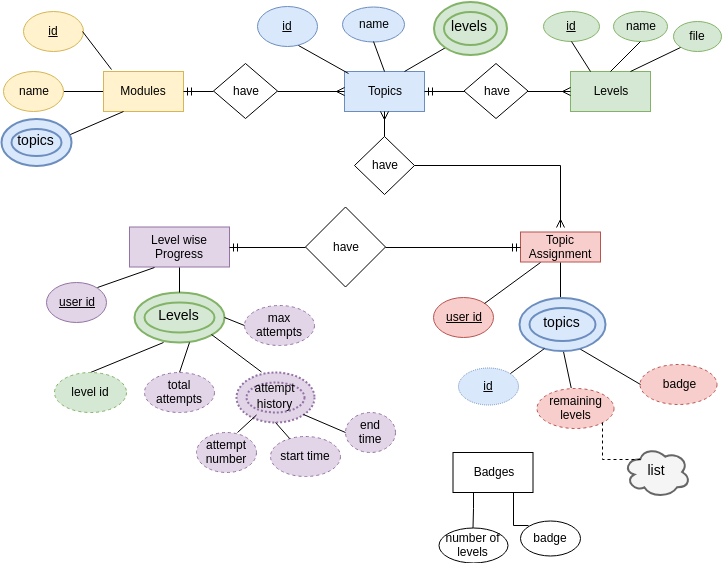
\includegraphics[width=\linewidth]{er.png}}
    \caption{ER Diagram}
    \label{fig:er}
\end{figure}
Users can see the all topics assigned to them and can select a topic to see all its levels. They will be able to see if they have completed the topic/ level or not and the number of retakes (in case of levels). The user can open any level at anytime and start the training. Once done, he/ she can mark the training as done. Once all the levels of a topic are completed at least once, the topic is marked completed. The user will also be given badges based on the levels of a topic completed.
\medskip\\
A group of users will be given the permission to upload trainings in the above specified format and assign topics to the users. Only these users can monitor the progress of all the users. They would be able to see all the assignments made and their status of completion. The badge for every topic, level wise and attempt wise completion level can also be seen.
\medskip\\
The module has different UI for two kind of users:
\begin{itemize}
    \item \textbf{Admin View: }The user with admin privileges can:
    \begin{itemize}
        \item add training material
        \item assign trainings to any user (admin or non admin)
        \item monitor the progress of the users who he assigns the trainings by knowing:
        \begin{itemize}
            \item the starting time for each level
            \item the ending time for each level
            \item number of retakes for each level
        \end{itemize}
    \end{itemize}
    Figure \ref{fig:s1} shows the process of adding and assigning training material and Figure \ref{fig:s3} shows the way progress is monitored.
    \item \textbf{Non Admin View: }The users without admin priveleges will be able to see only the trainings that they are assigned along with their status of completion and if started, the starting time, if completed, the time of completion and the number of retakes, if any. Figure \ref{fig:s2} shows the complete process of employee training.
\end{itemize}
\begin{figure}
    \centering
    \fbox{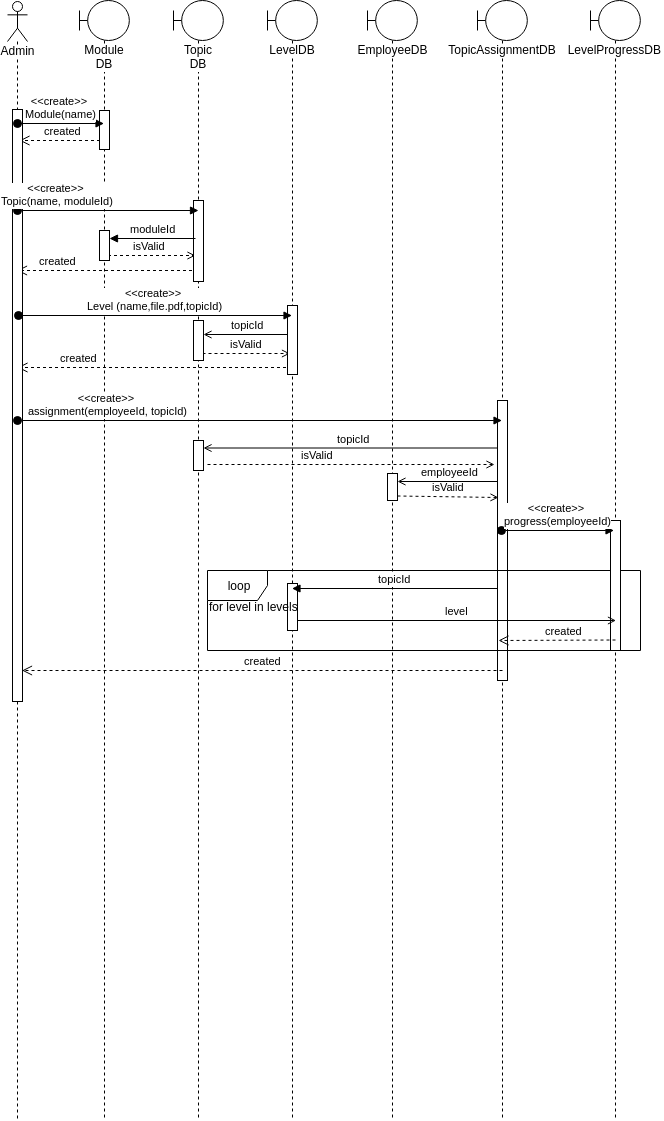
\includegraphics[trim={0 15cm 0 0},clip, width=\linewidth]{DBCreation.png}}
    \caption{Sequence Diagram for Adding and Assigning Training Material}
    \label{fig:s1}
\end{figure}
\begin{figure}
    \centering
    \fbox{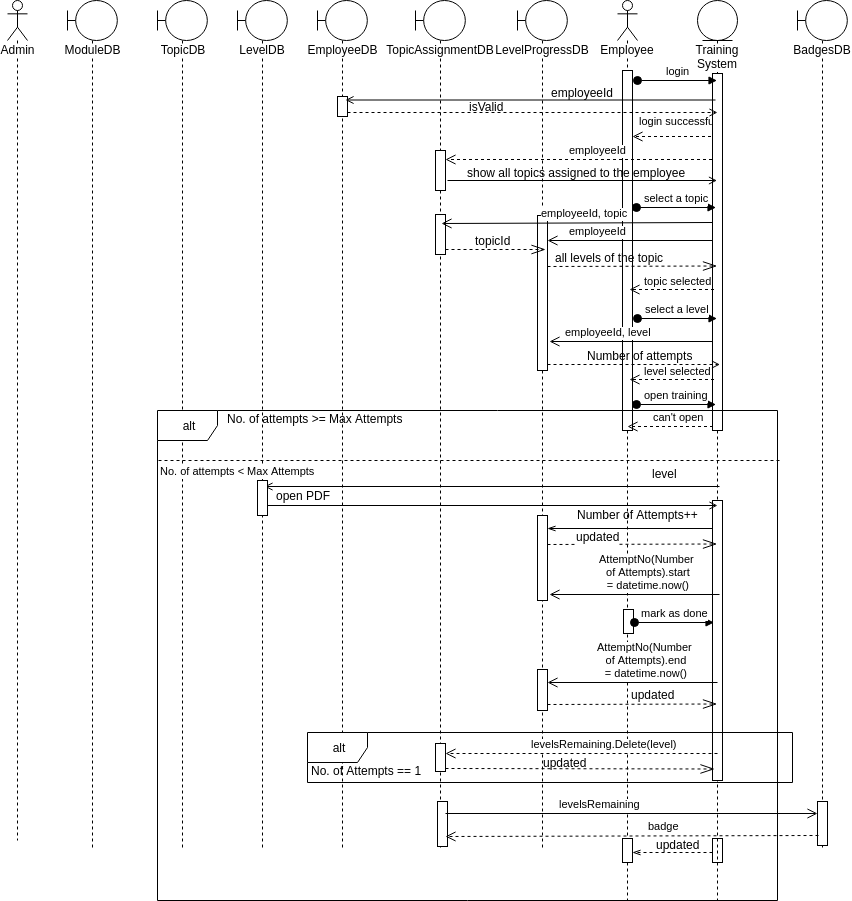
\includegraphics[width=\linewidth]{EmployeeTraining.png}}
    \caption{Sequence Diagram for Employee Training Process}
    \label{fig:s2}
\end{figure}
\begin{figure}
    \centering
    \fbox{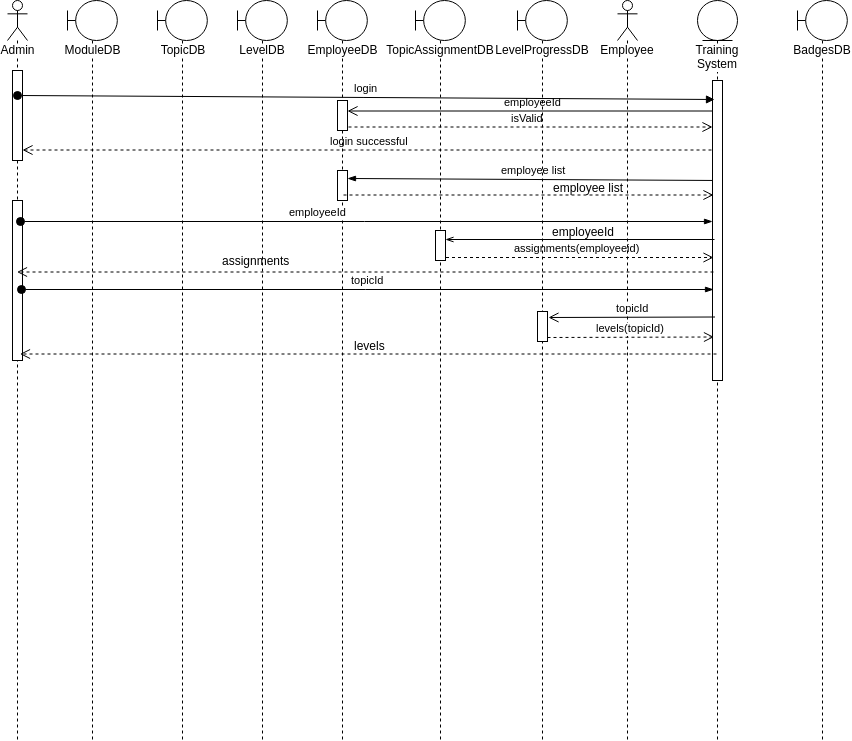
\includegraphics[trim={0 3cm 0 0},clip,width=\linewidth]{ProgressMonitor.png}}
    \caption{Sequence Diagram for Progress Monitor}
    \label{fig:s3}
\end{figure}

\newpage
\section{TOOLS AND TECHNOLOGY USED}
\hrule
\vspace*{5mm}
The tools and technologies used for the application can be refered from the Table \ref{tab:tech}. It is better to have separate frameworks handling the backend and frontend of the application. We use use Python-Eve for creating the APIs of our application and React for building its user interface. The details are as follows:

\begin{table}[ht]
\centering
\caption{Summary of Tools and Technologies Used} 
\begin{tabular}{|c|c|} 
\hline
 \multirow{5}{*}{\textbf{Languages}}&Python\\&JavaScript\\&HTML\\&CSS\\&ES6\\
 \hline
 \multirow{2}{*}{\textbf{Frameworks}}&Python-Eve (version 0.8.1)\\& React (version 16.4) \\ 
 \hline
 \textbf{Database} & MongoDB (version 3.6) \\
\hline
 \textbf{ORM} & Cerberus\\
\hline
\end{tabular}
\label{tab:tech}
\end{table} 

\subsection{Python-Eve}
Eve is an open source Python REST API framework designed for human beings \cite{bworld}. It allows to effortlessly build and deploy highly customizable, fully featured RESTful Web Services. Eve is powered by Flask and Cerberus and it offers native support for MongoDB data stores. Support for SQL, Elasticsearch and Neo4js backends is provided by community extensions. This application sticks to the default support of MongoDB for data storage and Flask and Cerberus for Object Reltional Modelling.
\medskip\\
Eve provides a robust, feature rich, REST-centered API implementation, and you just need to configure your API settings and behavior, plug in your datasource, and you’re good to go. 

\subsection{MongoDB}
MongoDB is a cross-platform document-oriented database program that used to be free and open-source but has since changed to a proprietary license \cite{mongo}(Server Side Public License). Classified as a NoSQL database program, MongoDB uses JSON-like documents with schemata. Main features of MongoDB are:
\begin{itemize}
    \item Ad hoc queries
    \item Indexing
    \item Replication
    \item Load Balancing
    \item File Storage
    \item Aggregation
    \item Serverside JavaScript Execution
    \item Capped Collections
    \item Transactions
\end{itemize}

\subsection{Cerberus}
Cerberus provides powerful yet simple and lightweight data validation functionality out of the box and is designed to be easily extensible, allowing for custom validation\cite{cerberus}. It has no dependencies and is thoroughly tested from Python 2.6 up to 3.5, PyPy and PyPy3. Unlike other validation tools, Cerberus will not halt and raise an exception on the first validation issue. The whole document will always be processed, and False will be returned if validation failed. You can then access the errors property to obtain a list of issues.

\subsection{React}
React (also known as React.js or ReactJS) is a JavaScript library for building user interfaces. It is maintained by Facebook and a community of individual developers and companies. React can be used as a base in the development of single-page or mobile applications\cite{react}. Complex React applications usually require the use of additional libraries for state management, routing, and interaction with an API.
\begin{itemize}
    \item \textbf{Declarative: }React makes it painless to create interactive UIs. Design simple views for each state in your application, and React will efficiently update and render just the right components when your data changes. Declarative views make your code more predictable and easier to debug.

    \item \textbf{Component-Based: }Component-Based: Build encapsulated components that manage their own state, then compose them to make complex UIs. Since component logic is written in JavaScript instead of templates, you can easily pass rich data through your app and keep state out of the DOM.
\end{itemize}

\newpage
\section{RESULTS AND DISCUSSIONS}
\hrule
\vspace*{5mm}

The application is successfully created, tested and deployed. It is included in Bridge and any employee with credentials to login Bridge can access the service. Admin privileges are currently provided to the intended users from the backend only and no arrangements are made to do so via the web. The trainings are visible in the website as a preview and can not be downloaded. This is necessary to ensure that the company's material is held within and not leaked. The badge assignment is not incorporated in the current version due to time constraint. The current versions supports addition of PDF format trainings grouped by topics and modules and their assignment to any other user. The assigned user can see all his trainings and access them any number of times he wants to. When completed, the assignee is notified with the starting and ending time of the training.

\newpage
\section{FUTURE SCOPE}
\hrule
\vspace*{5mm}
Following things are in the pipeline for this module:
\begin{itemize}
    \item \textbf{Interactive Training: }This is an extensive element that will revamp the complete look of the service. Instead of importing the trainings from some other source, we aim to prepare the training lessons internally within the service itself. This will not only eliminate dependency on multiple platforms but also enhance content security. Also, interactive buttons and slideshow elements can be added to make the lesson interesting.
    \item \textbf{Adding Quiz: }To test the trainee's skill and maintain a level of seriousness towards the process, quizes can be added after every section. This can be done only if interactive training lessons can be created. The quizes can further be used to give badges to the trainees and make the service engaging.
\end{itemize}

\newpage
\section{REFERENCES}
\hrule
\vspace*{5mm}
\bibliographystyle{IEEEtran}
\bibliography{refer} 

\iffalse
\begin{itemize}
  \cite{}
\end{itemize}
\fi


\end{document}
